\section{Results}
\label{sec:results}

More than 41000 strides have been extracted from the data, which resulted in more than 82000 hoof-on and hoof-off moments for the right front hoof and right hind hoof in total. The number of strides per gait is presented in Table \ref{strides_per_gait}. The estimation errors of the trained models in all gaits are presented in Figure \ref{models_result_fig} (top plot). In addition, the performances of the best performing models for front and hind hoof-on and hoof-off (which were the models based on front limb \gls{imu} and hind limb \gls{imu}) within all gaits are also displayed in Figure \ref{models_result_fig} (the four bottom plots). In Table \ref{results_of_models}, all of the models accuracy results presented in Figure \ref{models_result_fig} were reported in numbers.

\begin{table}[!htbp] 
    \centering
    \caption{Number of strides per gait}% Add 'table' caption
    \resizebox{0.85\linewidth}{!}{%
    \begin{tabular}{lccccccc}
    \toprule
 \textbf{Gait} & Walk & Trot & Canter & Passage & Piaffe & Unlabeled  & Total \\
\midrule
\textbf{Number of strides} & 4600  & 7800 & 10400 & 1900 & 1500 & 14800  & 41000 \\
\bottomrule
 \label{strides_per_gait}
\end{tabular}}
\end{table}


\begin{sidewaystable}[!htbp] 
    \centering
    \caption{Performance of the estimation models in two units: time (milliseconds) and timestep (1 timestep = 5 milliseconds). Positive value:  estimation delay, negative value:  early estimation.}% Add 'table' caption
    \resizebox{\linewidth}{!}{%
    \begin{tabular}{p{3cm}p{2cm}p{2cm}p{2cm}p{1.5cm}p{1.5cm}p{1.5cm}p{1.5cm}p{1.5cm}p{1.5cm}p{1.5cm}}
    \toprule


\multicolumn{1}{l}{\textbf{Input IMU}}        & \multicolumn{1}{l}{\textbf{Output IMU}}                    & \multicolumn{1}{l}{\textbf{Hoof-on/off}} & \multicolumn{1}{l}{\textbf{Unit}}         & \multicolumn{7}{c}{\textbf{Error (= mean ± standard deviation)}}                                                \\
          \cmidrule(lr){5-11}
                                  &                                                &                              &                               & \textbf{All gaits}                       & \textbf{Walk}                            & \textbf{Trot}                            & \textbf{Canter}                          & \textbf{Passage}                          & \textbf{Piaffe}                          & \textbf{Unlabeled}   \\
                                  \midrule
\multicolumn{1}{l}{Right front limb} & \multicolumn{1}{l}{Front hoof}                    & Hoof-on                      & Time (ms)                     & 0.6 ± 9.0                       & -0.2 ± 8.6                      & 1.6 ± 8.4                       & 0.1 ± 8.8                       & 0.8 ± 9.9                        & 0.8 ± 9.4                       & 0.6 ± 8.8   \\
                                  &                                                & Hoof-on                      & Timestep                     & 0 ± 2                           & 0 ± 2                           & 0 ± 2                           & 0 ± 2                           & 0 ± 2                            & 0 ± 2                           & 0 ± 2       \\
                                  &                                                & Hoof-off                     & Time (ms)                     & 0.0 ± 6.0                       & -0.1 ± 5.9                      & 0.1 ± 6.3                       & -0.3 ± 5.6                      & 0.2 ± 6.1                        & 0.1 ± 5.9                       & -0.1 ± 6.0  \\
                                  &                                                & Hoof-off                     & Timestep                      & 0 ± 1                           & 0 ± 1                           & 0 ± 1                           & 0 ± 1                           & 0 ± 1                            & 0 ± 1                           & 0 ± 1       \\
                                  \midrule
\multicolumn{1}{l}{Withers}          & \multicolumn{1}{l}{Front hoof}                    & Hoof-on                      & Time (ms)                     & -0.2 ± 21.0                     & -0.2 ± 16.9                     & -0.3 ± 19.4                     & 0.1 ± 22.9                      & -0.2 ± 24.0                      & -0.2 ± 20.9                     & -0.1 ± 21.0 \\
                                  &                                                & Hoof-on                      & Timestep                      & 0 ± 4.0                         & 0 ± 3                           & 0 ± 4                           & 0 ± 5                           & 0 ± 5                            & 0 ± 4                           & 0 ± 4       \\
                                  &                                                & Hoof-off                     & Time (ms)                     & -2.8 ± 17.0                     & -1.5 ± 13.7                     & -3.2 ± 15.5                     & -3.3 ± 18.5                     & -3.0 ± 19.9                      & -3.4 ± 17.0                     & -2.9 ± 16.8 \\
                                  &                                                & Hoof-off                     & Timestep                      & -1 ± 3                          & 0 ± 3                           & -1 ± 3                          & -1 ± 4                          & -1 ± 4                           & -1 ± 3                          & -1 ± 3      \\
                                  \midrule
\multicolumn{1}{l}{Right hind limb}  & \multicolumn{1}{l}{Hind hoof}                     & Hoof-on                      & Time (ms)                     & 6.5 ± 16.0                      & -4.7 ± 13.6                     & -5.4 ± 14.6                     & -7.2 ± 17.0                     & -9.0 ± 18.3                      & -6.5 ± 16.1                     & -6.4 ± 16.3 \\
                                  &                                                & \multicolumn{1}{l}{Hoof-on}  & \multicolumn{1}{l}{Timestep}  & \multicolumn{1}{l}{-1 ± 3}      & \multicolumn{1}{l}{-1 ± 3}      & \multicolumn{1}{l}{-1 ± 3}      & \multicolumn{1}{l}{-1 ± 3}      & \multicolumn{1}{l}{-2 ± 4}       & \multicolumn{1}{l}{-1 ± 3}      & -1 ± 3      \\
                                  &                                                & \multicolumn{1}{l}{Hoof-off} & \multicolumn{1}{l}{Time (ms)} & \multicolumn{1}{l}{5.6 ± 13.0}  & \multicolumn{1}{l}{3.3 ± 11.3}  & \multicolumn{1}{l}{4.6 ± 12.1}  & \multicolumn{1}{l}{6.6 ± 13.6}  & \multicolumn{1}{l}{7.6 ± 15.0}   & \multicolumn{1}{l}{6.4 ± 12.7}  & 5.6 ± 12.4  \\
                                  &                                                & \multicolumn{1}{l}{Hoof-off} & \multicolumn{1}{l}{Timestep}  & \multicolumn{1}{l}{1 ± 3}       & \multicolumn{1}{l}{1 ± 2}       & \multicolumn{1}{l}{1 ± 2}       & \multicolumn{1}{l}{1 ± 3}       & \multicolumn{1}{l}{2 ± 3}        & \multicolumn{1}{l}{1 ± 3}       & 1 ± 2       \\
                                  \midrule
\multicolumn{1}{l}{Sacrum}           & \multicolumn{1}{l}{Hind hoof} & \multicolumn{1}{l}{Hoof-on}  & \multicolumn{1}{l}{Time (ms)} & \multicolumn{1}{l}{-8.7 ± 29.0} & \multicolumn{1}{l}{-6.2 ± 24.7} & \multicolumn{1}{l}{-6.9 ± 27.3} & \multicolumn{1}{l}{-8.0 ± 29.8} & \multicolumn{1}{l}{-13.6 ± 32.1} & \multicolumn{1}{l}{-7.7 ± 29.1} & -7.5 ± 28.8 \\
                                  & \multicolumn{1}{l}{}                           & \multicolumn{1}{l}{Hoof-on}  & \multicolumn{1}{l}{Timestep}  & \multicolumn{1}{l}{-2 ± 6}      & \multicolumn{1}{l}{-1 ± 5}      & \multicolumn{1}{l}{-1 ± 5}      & \multicolumn{1}{l}{-2 ± 6}      & \multicolumn{1}{l}{-3 ± 6}       & \multicolumn{1}{l}{-2 ± 6}      & -2 ± 6      \\
                                  & \multicolumn{1}{l}{}                           & \multicolumn{1}{l}{Hoof-off} & \multicolumn{1}{l}{Time (ms)} & \multicolumn{1}{l}{7.9 ± 25.0}  & \multicolumn{1}{l}{5.5 ± 21.7}  & \multicolumn{1}{l}{7.8 ± 24.1}  & \multicolumn{1}{l}{7.9 ± 26.5}  & \multicolumn{1}{l}{9.3 ± 26.8}   & \multicolumn{1}{l}{8.2 ± 25.0}  & 8.0 ± 24.7  \\
                                  & \multicolumn{1}{l}{}                           & \multicolumn{1}{l}{Hoof-off} & \multicolumn{1}{l}{Timestep}  & \multicolumn{1}{l}{2 ± 5}       & \multicolumn{1}{l}{1 ± 4}       & \multicolumn{1}{l}{2 ± 5}       & \multicolumn{1}{l}{2 ± 5}       & \multicolumn{1}{l}{2 ± 5}        & \multicolumn{1}{l}{2 ± 5}       & 2 ± 5\\  
                                  \bottomrule
                                   \label{results_of_models}
\end{tabular}}
\end{sidewaystable}

\begin{figure}[htbp]
\centering
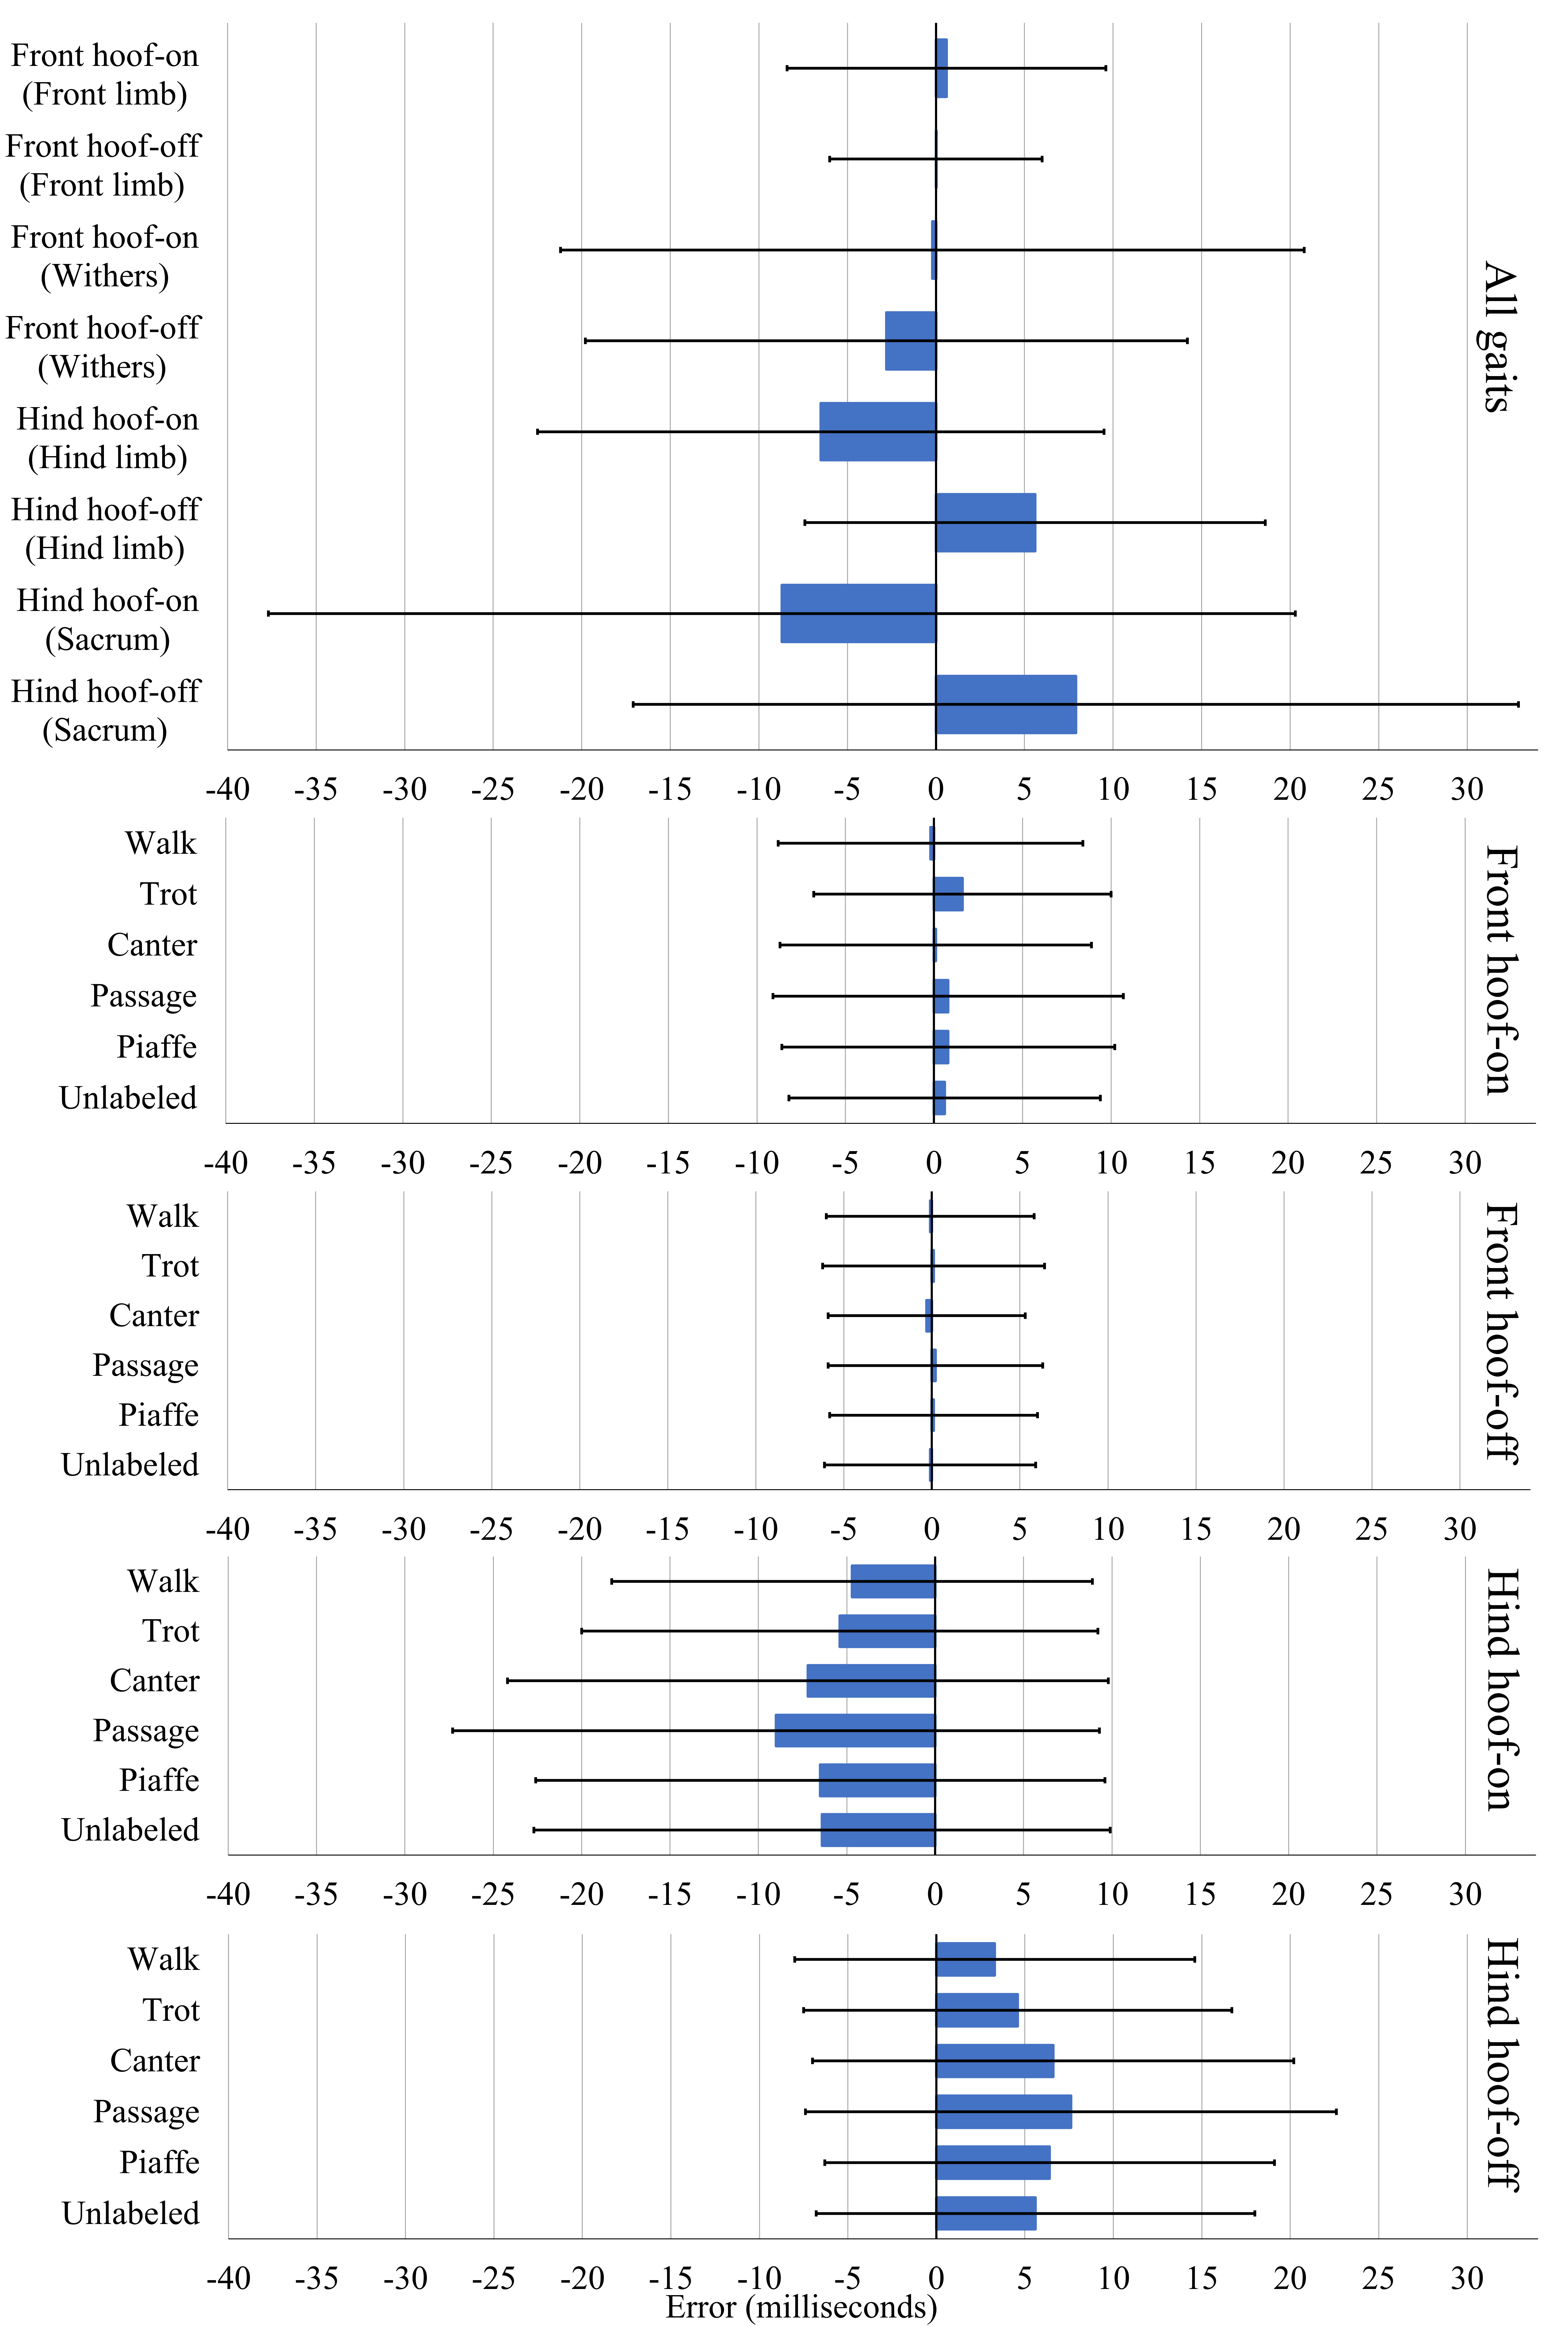
\includegraphics[width=.88\linewidth]{chapters/Step/figures/model_performances_step.png}
\caption{The Performances of the estimation models. Top: Performance of the models within all gaits per \gls{imu}. Second: Performance (per gait) of the front hoof-on model trained on front-limb \gls{imu}. Third: Performance (per gait) of the front hoof-off model trained on front-limb \gls{imu}. Fourth: Performance (per gait) of the hind hoof-on model trained on hind-limb \gls{imu}. Fifth: Performance (per gait) of the hind hoof-off model trained on hind-limb \gls{imu}. The bars and the error bars indicate the accuracy (mean) and precision (standard deviation) of estimation errors, respectively.}
\label{models_result_fig}
\end{figure}


It can be inferred from the top plot of Figure \ref{models_result_fig} that the model based on front limb \gls{imu} yielded the best accuracy and precision for both hoof-on and hoof-off, with -0.2 and -0.1 ms accuracy and 9.0 and 6.0 ms precision, respectively. Between upper-body mounted \gls{imu}s, the hoof-on and hoof-off models based on withers \gls{imu} presented lower errors (-0.2 ± 21.0 and -2.8 ± 17.0 ms) than sacrum \gls{imu} for hind hoof-on (-8.7 ± 29.0 ms) and -off (7.9 ± 25.0 ms). A positive and negative value can be defined as an estimation delay and an early estimation of the moment, respectively.

All the models yielded the best performance when W and batch size were 100 and 32, respectively. The tuned value of other hyperparameters, learning rate and dropout rate, were different among the models. The learning rate varied between 0.0001 and 0.0005, while the dropout rate values were 0.2, 0.4, and 0.6. The values of hyperparameters that resulted in highest accuracy for each model were reported in Table \ref{hyperparameters}.

\begin{table}[!htbp] 
    \centering
    \caption{Number of strides per gait}% Add 'table' caption
    \resizebox{0.8\linewidth}{!}{%
    \begin{tabular}{lcccc}
    \toprule
 \textbf{Input \gls{imu}} & \textbf{Output \gls{imu}} & \textbf{Hoof-on/off} & \textbf{Learning rate} & \textbf{Dropout rate}  \\
\midrule
Right front limb & Front hoof  & Hoof-on & 0.0001 & 0.6\\
 &  & Hoof-off & 0.0005 & 0.4\\
Withers & Front hoof  & Hoof-on & 0.0001 & 0.4\\
 &   & Hoof-off & 0.0005 & 0.4\\
Right hind limb & Hind hoof  & Hoof-on & 0.0001 & 0.6\\
 &  & Hoof-off & 0.0005 & 0.4\\
 Sacrum & Hind hoof  & Hoof-on & 0.0005 & 0.2\\
 &  & Hoof-off & 0.0005 & 0.4\\


\bottomrule
 \label{hyperparameters}
\end{tabular}}
\end{table}

According to the results, the precision increased and decreased respectively as the models (except for the right front limb model) estimated the hoof-on and hoof-off during faster natural gaits, from walk to canter (speed of cantering > speed of trotting > speed of walking). In artificial gaits, both accuracy and precision were lower in piaffe compared to passage. Therefore, we achieved the lowest and highest error during walk and passage, respectively.

Figure \ref{literature_compare_fig} demonstrated and Table \ref{literature_compare_} reported the performance results of the current study models in comparison to the results of the state-of-the-art methods \cite{adsd1,sapone_2020_comparison}. Although the method was only based on front and hind limbs \gls{imu}s (as the input), models based on withers and sacrum \gls{imu}s were also presented for comparison (based on the output \gls{imu}s) of models performances in terms of \gls{imu} placement on the body.






\begin{figure}[htbp]
\centering
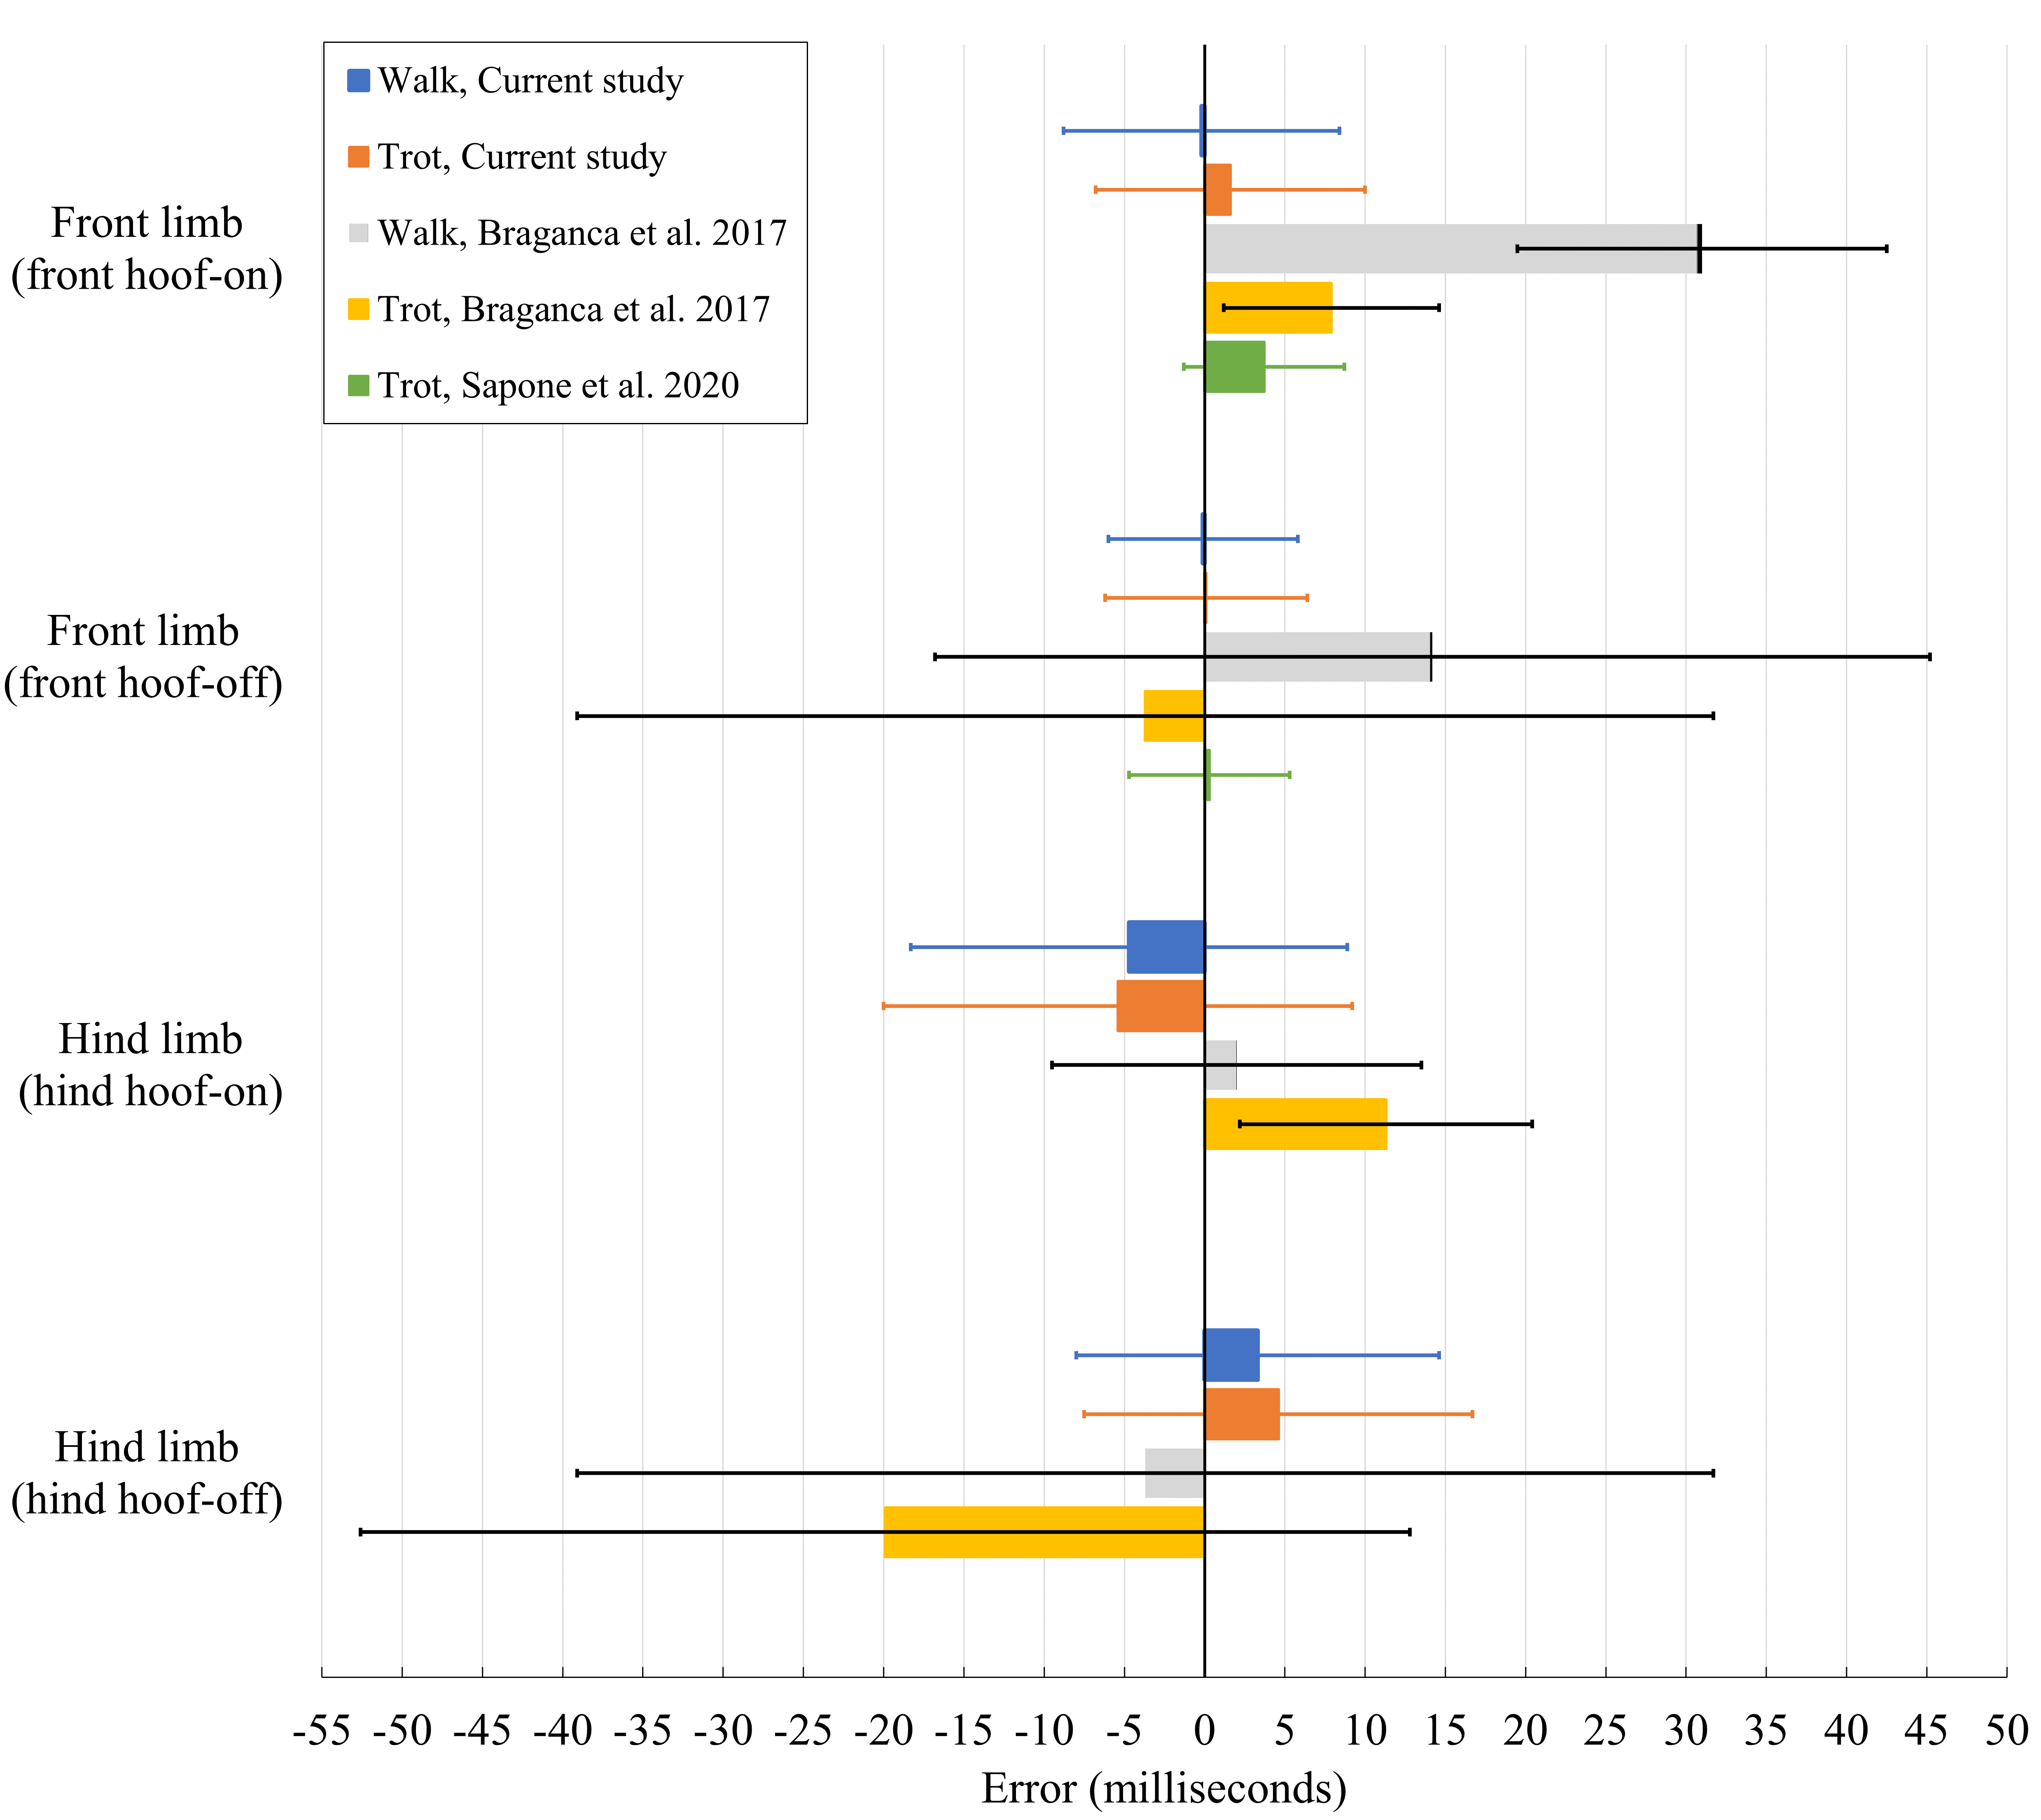
\includegraphics[width=.95\linewidth]{chapters/Step/figures/Studies_step.png}
\caption{The comparison between estimation models of the current study and the literature. The bars and the error bars indicate the accuracy (mean) and precision (standard deviation) of the estimation models, respectively.}
\label{literature_compare_fig}
\end{figure}


\begin{table}[!htbp] 
    \centering
    \caption{Comparison of the outcome of estimation models from the current study and the literature 
(positive value:  estimation delay, negative value:  early estimation).}% Add 'table' caption
    \resizebox{\linewidth}{!}{%
    \begin{tabular}{llccccc}
    \toprule

&                   & \multicolumn{2}{c}{\textbf{Current study}}         & \multicolumn{2}{c}{\textbf{Bragan\c{c}a et al. \cite{adsd1}}} & \multicolumn{1}{c}{\textbf{Sapone et al. \cite{sapone_2020_comparison}}}\\
 
          \cmidrule(lr){3-4} \cmidrule(lr){5-6} \cmidrule(lr){7-7}
 
 
\multicolumn{1}{l}{\textbf{Input IMU}}        & \multicolumn{1}{c}{\textbf{Output}}  &  \textbf{Walk} & \textbf{Trot} & \textbf{Walk} & \textbf{Trot} & \textbf{Trot}\\

\midrule

Right front limb & Front hoof-on& -0.2 ± 8.6 & 1.6 ± 8.4 & 0.3 ± 11.5 & 7.9 ± 6.7 & 3.7 ± 17.0\\
                               
 & Front hoof-off & -0.2 ± 16.9 & -0.3 ± 19.4 & 14.2 ± 31.0 & -3.7 ± 35.4 & 0.3 ± 15.4\\
 
 \midrule
 
 Withers & Front hoof-on& -0.2 ± 16.9 & -0.3 ± 19.4 &- &- &- \\
 
   & Front hoof-off & -1.5 ± 13.7 & -3.2 ± 15.5 &- & -& -\\
 
 \midrule
 
 Right hind limb & Hind hoof-on & -4.7 ± 13.6 & -5.4 ± 14.6 & 2.0 ± 11.5 & 11.3 ± 9.1 & -\\
 
  &  Hind hoof-off & 3.3 ± 11.3 & 4.6 ± 12.1 & -3.7 ± 35.4 & -19.9 ± 32.7 & -\\
  
  \midrule
  
  Sacrum & Hind hoof-on & -6.2 ± 24.7 & -6.9 ± 27.3 &- &- &-\\
 
   & Hind hoof-off & 5.5 ± 21.7 & 7.8 ± 24.1 & - & - & -\\
         \bottomrule
                                   \label{literature_compare_}
\end{tabular}}
\end{table}